\documentclass[11pt,a4paper]{article}
\usepackage[T1]{fontenc}
\usepackage[utf8]{inputenc}
\usepackage[a4paper,margin=2.4cm]{geometry}
\usepackage[compat=1.1.0]{tikz-feynman}
\usepackage{booktabs,caption,float}
\usepackage{setspace}
\captionsetup{font=small,labelfont=bf}
\title{Supplementary Material: Feynman-Diagram Notation of the LOKLOK Experimental Processes}
\author{Sherif Mohamed Abd Elmonem Rashwan \\ Ahram Canadian University, Faculty of Mass Communication}
\date{November 2026}
\begin{document}
\maketitle
\begin{center}\small Companion supplement to the master's thesis ``The Social Media Radio Innovation and Its Impact on University Students' Ratings: An Exploratory Study.''\end{center}

\section*{Purpose and convention}
The diagrams in this supplement express the LOKLOK experimental processes in the
diagrammatic notation of particle physics. They are pedagogical supplements: they
borrow the visual grammar of Feynman diagrams to make mechanism dependencies,
interaction orders, and measurement points explicit. Nothing in them is a claim
about physics; the Hamiltonian analogy in the thesis carries the same caveat.

\begin{table}[H]\centering\small
\caption{Line and vertex conventions}
\begin{tabular}{@{}ll@{}}
\toprule
Symbol & Meaning in the LOKLOK reading \\
\midrule
Solid arrow line (fermion) & Agent line: student, listener, broadcaster, viewpoint, or content; the arrow gives the direction of judgment or content flow \\
Wiggly line (photon) & Audio signal, broadcast, reflection prompt, cooling radiation, or a measurement response \\
Curly line (gluon) & Platform mechanism exchange: diversity constraint, LOKLOK filters, gate self-interaction, evidence loop \\
Dashed line (scalar) & Misinformation before and corrected content after moderation \\
Filled circle (blob) & Algorithmic filter or update: MORE, ERIC, BRS evidence update, Zewail gate, GRM-IRT detector \\
Crossed vertex & Randomization point or measurement point separating latent from observed \\
\bottomrule
\end{tabular}
\end{table}

\section*{The ten situations}

\subsection*{D1. Listening as absorption}
\begin{figure}[H]
\centering
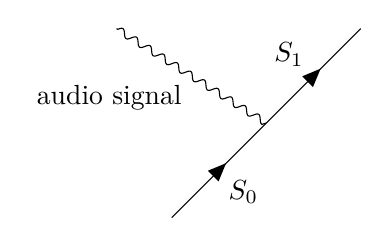
\begin{tikzpicture}
\begin{feynman}
\vertex (a) at (-1.2,-1.2);
\vertex (b) at (1.2,1.2);
\vertex (v) at (0,0);
\vertex (s) at (-1.9,1.2);
\diagram*{
(s) -- [photon, edge label'=audio signal] (v),
(a) -- [fermion, edge label'=$S_0$] (v) -- [fermion, edge label=$S_1$] (b),
};
\end{feynman}
\end{tikzpicture}

\caption{D1. Listening as absorption}
\end{figure}
A broadcaster emits an audio signal (photon). The listener line (fermion) absorbs it at a vertex and continues with an updated judgment state S0 to S1. This is the elementary process every other diagram composes.

\subsection*{D2. EST-P1: structural credibility through the BRS anchor}
\begin{figure}[H]
\centering
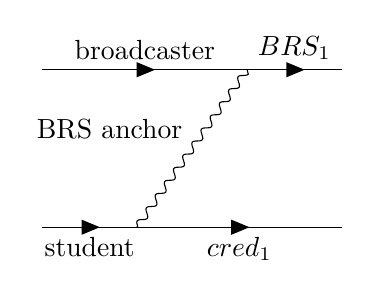
\begin{tikzpicture}
\begin{feynman}
\vertex (a) at (-1.9,-1.0);
\vertex (b) at (1.9,-1.0);
\vertex (c) at (-1.9,1.0);
\vertex (d) at (1.9,1.0);
\vertex (v1) at (-0.7,-1.0);
\vertex (v2) at (0.7,1.0);
\diagram*{
(a) -- [fermion, edge label'=student] (v1) -- [fermion, edge label'=$cred_1$] (b),
(c) -- [fermion, edge label=broadcaster] (v2) -- [fermion, edge label=$BRS_1$] (d),
(v1) -- [photon, edge label=BRS anchor] (v2),
};
\end{feynman}
\end{tikzpicture}

\caption{D2. EST-P1: structural credibility through the BRS anchor}
\end{figure}
A student and a broadcaster exchange a BRS anchor (photon) at a scattering vertex. After the exchange the student carries credibility cred1 and the broadcaster carries reputation BRS1: architecture enters as the exchanged field, not as an external parameter.

\subsection*{D3. EST-P2: the diversity constraint in MORE}
\begin{figure}[H]
\centering
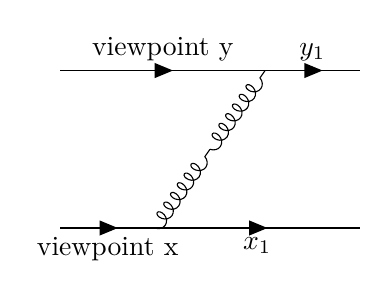
\begin{tikzpicture}
\begin{feynman}
\vertex (a) at (-1.9,-1.0);
\vertex (b) at (1.9,-1.0);
\vertex (c) at (-1.9,1.0);
\vertex (d) at (1.9,1.0);
\vertex (v1) at (-0.7,-1.0);
\vertex (v2) at (0.7,1.0);
\vertex[blob] (g) at (0,0);
\diagram*{
(a) -- [fermion, edge label'=viewpoint x] (v1) -- [fermion, edge label'=$x_1$] (b),
(c) -- [fermion, edge label=viewpoint y] (v2) -- [fermion, edge label=$y_1$] (d),
(v1) -- [gluon] (g) -- [gluon] (v2),
};
\end{feynman}
\end{tikzpicture}

\caption{D3. EST-P2: the diversity constraint in MORE}
\end{figure}
Two viewpoints exchange a diversity constraint through the MORE filter (blob), drawn as a gluon exchange. The blob makes the constraint local to the platform; the viewpoints emerge correlated rather than independent.

\subsection*{D4. The Zewail-inspired attention gate}
\begin{figure}[H]
\centering
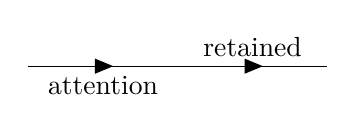
\begin{tikzpicture}
\begin{feynman}
\vertex (a) at (-1.9,0);
\vertex (b) at (1.9,0);
\vertex[blob] (g) at (0,0);
\diagram*{
(a) -- [fermion, edge label'=attention] (g) -- [fermion, edge label=retained] (b),
(g) -- [gluon, half left, looseness=1.5, edge label'=$\tau$ gate] (g),
};
\end{feynman}
\end{tikzpicture}

\caption{D4. The Zewail-inspired attention gate}
\end{figure}
An attention line passes through the gate (blob) and emerges retained. The gluon loop on the blob is the gate self-interaction, parameterized by the dephasing time tau: the loop stands for the time-resolved retention that a static filter does not have.

\subsection*{D5. Algorithmic cooling of echo}
\begin{figure}[H]
\centering
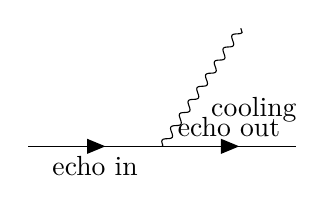
\begin{tikzpicture}
\begin{feynman}
\vertex (a) at (-1.7,0);
\vertex (b) at (1.7,0);
\vertex (v) at (0,0);
\vertex (k) at (1.0,1.5);
\diagram*{
(a) -- [fermion, edge label'=echo in] (v) -- [fermion, edge label=echo out] (b),
(v) -- [photon, edge label'=cooling] (k),
};
\end{feynman}
\end{tikzpicture}

\caption{D5. Algorithmic cooling of echo}
\end{figure}
An echo line radiates a cooling photon at a vertex, like bremsstrahlung. The radiated energy is removed from the echo state, which is the diagrammatic form of the cooling step.

\subsection*{D6. The main experiment: G0 to G1}
\begin{figure}[H]
\centering
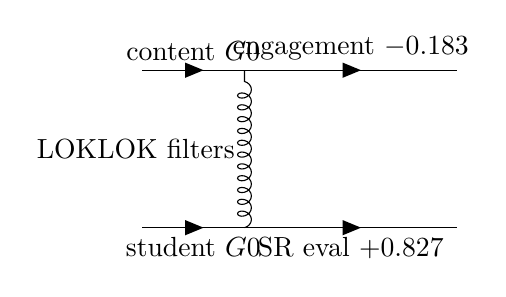
\begin{tikzpicture}
\begin{feynman}
\vertex (s1) at (-2.0,-1.0);
\vertex (s2) at (2.0,-1.0);
\vertex (c1) at (-2.0,1.0);
\vertex (c2) at (2.0,1.0);
\vertex (v1) at (-0.7,-1.0);
\vertex (v2) at (-0.7,1.0);
\diagram*{
(s1) -- [fermion, edge label'=student $G0$] (v1) -- [fermion, edge label'=SR eval $+0.827$] (s2),
(c1) -- [fermion, edge label=content $G0$] (v2) -- [fermion, edge label=engagement $-0.183$] (c2),
(v1) -- [gluon, edge label=LOKLOK filters] (v2),
};
\end{feynman}
\end{tikzpicture}

\caption{D6. The main experiment: G0 to G1}
\end{figure}
A student line and a content line enter from G0 and exchange the LOKLOK filter field (gluon). The outgoing states carry the headline observables: SR eval +0.827 and engagement -0.183. The diagram makes the interaction order explicit: the platform acts between the student and the content, never on them separately.

\subsection*{D7. The BRS evidence update}
\begin{figure}[H]
\centering
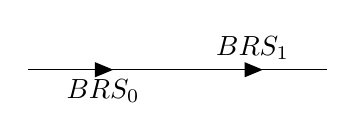
\begin{tikzpicture}
\begin{feynman}
\vertex (a) at (-1.9,0);
\vertex (b) at (1.9,0);
\vertex[blob] (g) at (0,0);
\diagram*{
(a) -- [fermion, edge label'=$BRS_0$] (g) -- [fermion, edge label=$BRS_1$] (b),
(g) -- [gluon, half left, looseness=1.5, edge label'=evidence] (g),
};
\end{feynman}
\end{tikzpicture}

\caption{D7. The BRS evidence update}
\end{figure}
A reputation line passes through an update blob. The gluon loop injects evidence at the blob: each loop order corresponds to one round of evidence-based revision, the diagrammatic form of the reputation contraction.

\subsection*{D8. ERIC moderation as a correction vertex}
\begin{figure}[H]
\centering
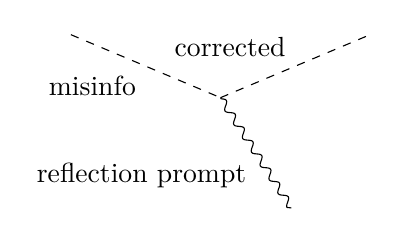
\begin{tikzpicture}
\begin{feynman}
\vertex (m) at (-1.9,0.8);
\vertex (c) at (1.9,0.8);
\vertex[blob] (v) at (0,0);
\vertex (p) at (0.9,-1.4);
\diagram*{
(m) -- [scalar, edge label'=misinfo] (v) -- [scalar, edge label=corrected] (c),
(v) -- [photon, edge label'=reflection prompt] (p),
};
\end{feynman}
\end{tikzpicture}

\caption{D8. ERIC moderation as a correction vertex}
\end{figure}
A misinformation line (scalar, dashed) enters the ERIC blob and leaves corrected. The radiated photon is the reflection prompt sent back to the user: moderation is drawn as an interaction, not as deletion.

\subsection*{D9. Randomized assignment as a branching vertex}
\begin{figure}[H]
\centering
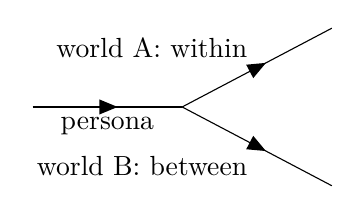
\begin{tikzpicture}
\begin{feynman}
\vertex[crossed dot] (x) at (0,0);
\vertex (i) at (-1.9,0);
\vertex (b1) at (1.9,1.0);
\vertex (b2) at (1.9,-1.0);
\diagram*{
(i) -- [fermion, edge label'=persona] (x),
(x) -- [fermion, edge label=world A: within] (b1),
(x) -- [fermion, edge label'=world B: between] (b2),
};
\end{feynman}
\end{tikzpicture}

\caption{D9. Randomized assignment as a branching vertex}
\end{figure}
A persona line splits at a crossed vertex into two worlds: within-persona assignment (A) and between-agent assignment (B). The crossing marks the randomization point, the only place where the two designs differ.

\subsection*{D10. GRM-IRT measurement}
\begin{figure}[H]
\centering
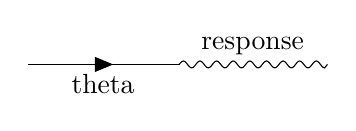
\begin{tikzpicture}
\begin{feynman}
\vertex (a) at (-1.9,0);
\vertex[crossed dot] (v) at (0,0);
\vertex[blob] (d) at (1.9,0);
\diagram*{
(a) -- [fermion, edge label'=theta] (v),
(v) -- [photon, edge label=response] (d),
};
\end{feynman}
\end{tikzpicture}

\caption{D10. GRM-IRT measurement}
\end{figure}
A latent trait line (theta) reaches a crossed measurement vertex and emits a response photon that the detector blob (GRM-IRT scoring of the NMLS and MCS batteries) absorbs. The cross separates the unobservable trait from the observed rating.

\end{document}